\noindent In this section, we apply Danzer's algorithm \cite{Danz02} to prove that every tiling in the tiling space of $\sigma_{n}$, for $n \in \{13, 17, 21\}$, has infinite local complexity.  
The main idea of the algorithm is to select a vertex in a misfit situation and then iterate the substitution along a line passing through this vertex. This procedure yields an infinite sequence of segments of distinct lengths, each corresponding to a unique edge type, and the non-Pisot property of the substitution factor plays a key role in establishing the unbounded growth of distinct lengths.

\begin{thm}
\label{thm:n-foldILC}
Every tiling in $\mathbb{X}_{\sigma_{13}}$ has infinite local complexity.
\end{thm}
\begin{proof}
Consider the edge type $P$ given in Figure~\ref{fig:iteration1}. Such an edge type is legal since a rotated copy of it occurs at the right corner of $\sigma_{13}(T_{13,1})$. Applying the substitution to $P$ produces a vertex in a misfit situation. We embed a copy of $\sigma_{13}(P)$ in the plane as follows (see Figure~\ref{fig:iteration1}): place the chosen misfit vertex at the origin $O$; align the edge of the tile $T$ containing this vertex (but not as one of its corners) along the $x$-axis; and position $T$ entirely within the upper half-plane.

\begin{figure}[H]
\centering
\includegraphics[width=0.8\textwidth]{ILCFig12.png}
			\caption{The image of the edge type $P$ under $\sigma_{13}$, with the misfit vertex placed at the origin and tile $T$ lying above the $x$-axis. (The color opacity has been adjusted to emphasize the segments.)}
\label{fig:iteration1}
\end{figure}

Let us denote by $A_1$ and $B_1$ the endpoints of the edge of the tile $T$ that contains the misfit vertex, as shown in the figure. Applying $\sigma_{13}$ to $\sigma_{13}(P)$ replaces the edge $\overline{A_1B_1}$ with a finite sequence of edges from substituted tiles in the upper half-plane. The total length of these edges is $\mu_{13} |\overline{A_1B_1}|$, where $|\overline{A_1B_1}|$ denotes the length of the edge. Since the origin lies between $A_1$ and $B_1$, one of these new edges must contain the origin. In Figure~\ref{fig:iteration2}, this edge is the base of a tile $T'$, with endpoints $A_2$ and $B_2$.


\begin{figure}[H]
\centering
\includegraphics[width=0.8\textwidth]{ILCFig13.png}
			\caption{Edges $\overline{A_1 B_1}$ and  $\overline{A_2 B_2}$.}
\label{fig:iteration2}
\end{figure}

Iterating the process yields a sequence of edges $(\overline{A_rB_r}){r \in \mathbb{N}}$, where each $\overline{A_rB_r}$ is the base of a tile lying in the upper half-plane and contained in $\sigma_{13}^r(P)$. As illustrated in Figures~\ref{fig:iteration1} and \ref{fig:iteration2}, which show the cases $r = 1$ and $r = 2$, the point $B_r$ is defined so that it lies strictly to the right of the origin. So $|\overline{OB_r}| > 0$ for every $r$.

We now associate to each edge $\overline{OB_r}$ a unique edge type $E_r$, defined as the pair of tiles that intersect along $\overline{OB_r}$ and both contain the origin. For example, $E_1 = \{T, T''\}$ and $E_2 = \{T', T'''\}$ (see Figure~\ref{fig:iteration2}). Since $\sigma_{13}$ is primitive, every edge type $E_r$ appears in every tiling $\mathcal{T} \in \mathbb{X}_{\sigma_{13}}$. Furthermore, if $|\overline{OB_{r_1}}| \neq |\overline{OB_{r_2}}|$ for some $r_1, r_2 \in \mathbb{N}$, then the corresponding edge types $E_{r_1}$ and $E_{r_2}$ are not equivalent. Therefore, if the values $|\overline{OB_r}|$ take infinitely many distinct values, the tiling $\mathcal{T}$ must contain infinitely many non-equivalent edge types, which implies $\mathcal{T}$ exhibits ILC. \\

So, in the following, we aim to show that the values $|\overline{OB_r}|$ take infinitely many distinct values. As a first step, we show that each length $|\overline{OB_r}|$ lies in $\mathbb{Z}[\mu_{13}]$ for all $r \in \mathbb{N}$. \\

We begin with the case $r=1$. We note that $|\overline{OB_1}|=|\overline{A_1B_1}|-|\overline{A_1O}|=s_{13,1}-(s_{13,4}+s_{13,6} )$ (see Figure~\ref{fig:iteration1}; $\overline{A_1B_1}$ is the base of the tile $T$ equivalent to $T_{13,1}$ in the upper half-plane, and $\overline{A_1O}$ is a composition of bases of tiles equivalent to $T_{13,4}$ and $T_{13,6}$ in the lower half-plane). By Lemma~\ref{lem:s_n,j}, we know that $s_{13,j} \in \mathbb{Z}[\mu_{13}]$ for each $j \in \{0,1,\ldots,6\}$. Thus, $|\overline{OB_1}| =s_{13,1}-(s_{13,4}+s_{13,6} ) \in \mathbb{Z}[\mu_{13}]$ by the closure property of $\mathbb{Z}[\mu_{13}]$.  

Now, for $r>1$, the length $|\overline{OB_r}|$ can be expressed using the recursive formula:

\begin{equation}
|\overline{OB_r}|=\mu_{13} |\overline{OB_{r-1}}|-t_r,           
\label{eq:recursion}
\end{equation}
\noindent where $t_r$ is the sum of finitely many prototile edge lengths. (The recursive formula is illustrated in Figure~\ref{fig:proofn=13} for $1< r \leq5$.  So $t_r \in \mathbb{Z}[\mu_{13}]$.) Therefore, since $|\overline{OB_1}|, \ t_r \in \mathbb{Z}[\mu_{13}]$, $|\overline{OB_r}|=\mu_{13}|\overline{OB_{r-1}}|-t_{r} \in \mathbb{Z}[\mu_{13}]$ by the closure property of $\mathbb{Z}[\mu_{13}]$.

\begin{figure}[H]
\centering
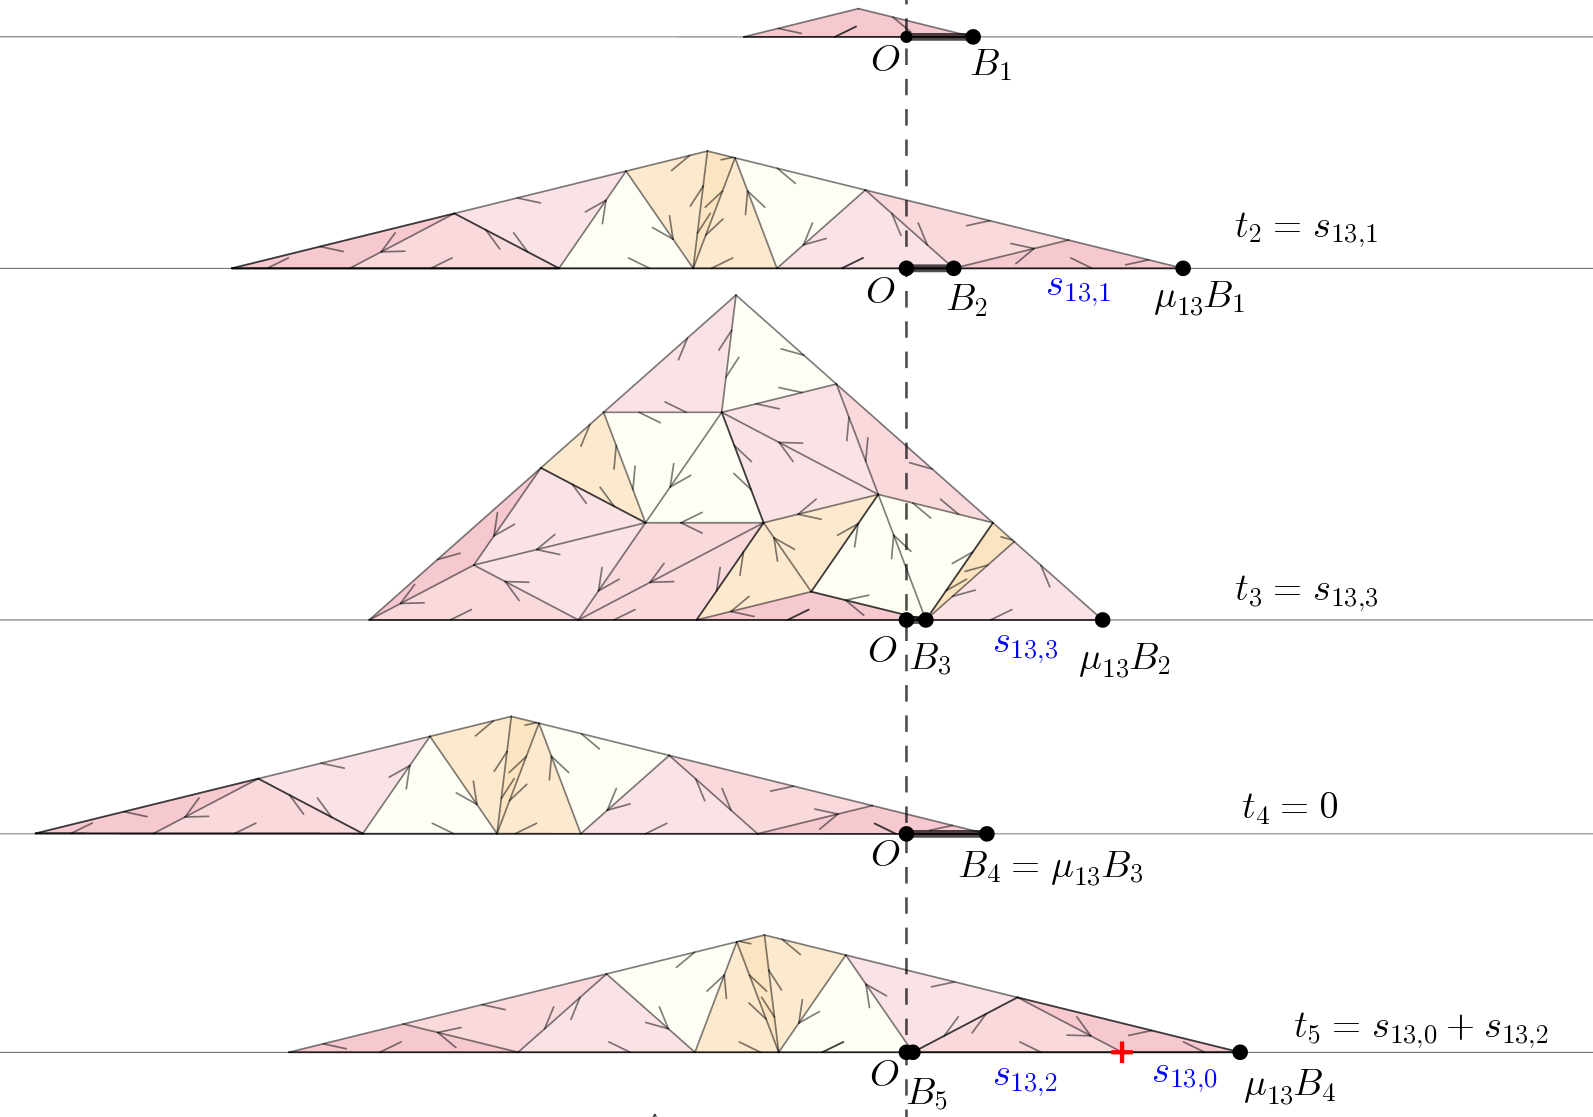
\includegraphics[width=0.8\textwidth]{ILCFig14.png}
			\caption{$|\overline{OB_r}|$, $r=1,2,3,4,5.$}
\label{fig:proofn=13}
\end{figure}

Let $w_r = (b_{r_0}, b_{r_1}, \dots, b_{r_5})^{\top} \in \mathbb{Z}^6$ be the coordinate vector of $|\overline{OB_r}|$. As mentioned ealier, multiplication by $\mu_{13}$ in $\mathbb{Z}[\mu_{13}]$ corresponds to left multiplication by the companion matrix $G_{13}$ of the minimal polynomial $g_{13}(x)$ in $\mathbb{Z}^6$. So in $\mathbb{Z}^6$, the recursive formula \ref{eq:recursion} is equivalent to

\begin{equation}
w_r=G_{13} w_{r-1}-u_r,
\label{eq:recursionvec}     	
\end{equation}

\noindent where $u_{r} \in \mathbb{Z}^6$ is the coordinate vector of $t_r$ in $\mathbb{Z}^6$.  To illustrate this, recall that $|\overline{OB_1}|=s_{13,1}-(s_{13,4}+s_{13,6})$ and Figure~\ref{fig:proofn=13} shows that $t_2=s_{13,1}$. From Table~\ref{tab:vectorrep}, we have 

$$
w_1 =y_{13,1}-(y_{13,4}+y_{13,6})=
\begin{bmatrix}
-4 \\ 1 \\ 10 \\ -3 \\ -4 \\ 1
\end{bmatrix}
-
\left(
\begin{bmatrix}
-5 \\ 0 \\ 16 \\ -5 \\ -8 \\ 2
\end{bmatrix}
+
\begin{bmatrix}
-1 \\ 5 \\ 4 \\ -6 \\ -3 \\ 1
\end{bmatrix}
\right)=\begin{bmatrix} 2 \\ -4 \\ -10 \\ 8 \\ 7 \\ -2\end{bmatrix}
 \quad \mbox{and} \quad u_{2} = y_{13,1}= \begin{bmatrix}
-4 \\ 1 \\ 10 \\ -3 \\ -4 \\ 1
\end{bmatrix}.
$$
So, 
\[
w_2 = G_{13} w_1 - u_2 = 
\begin{bmatrix}
0 & 0 & 0 & 0 & 0 & 1 \\
1 & 0 & 0 & 0 & 0 & 1 \\
0 & 1 & 0 & 0 & 0 & -5 \\
0 & 0 & 1 & 0 & 0 & -4 \\
0 & 0 & 0 & 1 & 0 & 6 \\
0 & 0 & 0 & 0 & 1 & 3 
\end{bmatrix}
\begin{bmatrix} 2 \\ -4 \\ -10 \\ 8 \\ 7 \\ -2\end{bmatrix} -
\begin{bmatrix} -4 \\ 1 \\ 10 \\ -3 \\ -4 \\ 1 \end{bmatrix} =
\begin {bmatrix} 2 \\-1 \\ -4 \\ 1 \\ 0 \\ 0 \end{bmatrix}.
\]

Since there is a one-to-one correspondence between the lengths $|\overline{OB_r}|$ and their coordinate vectors $w_r$, we can establish ILC by showing that $w_r$ takes infinitely many distinct values. For this purpose, it is more convenient to work with the diagonal matrix $\widetilde{G}_{13} = A^{-1} G_{13} A$ (see \ref{eq:Gtilde}) rather than $G_{13}$. As described by Danzer in \cite{Danz02}, a key advantage of this approach is that the recursive process can be applied directly to the entries of the vectors.

By left-multiplying the recursion $w_r = G_{13} w_{r-1} - u_r$ by $A^{-1}$ and inserting the identity $I = A A^{-1}$ between $G_{13}$ and $w_{r-1}$, the recursion \eqref{eq:recursionvec} becomes
\begin{equation}
\label{eq:recursionsecond}
w_r' \;=\; \widetilde{G}_{13}\, w_{r-1}' \;-\; u_r',
\end{equation}
where $w_r'= A^{-1} w_r$, $u_r'= A^{-1} u_r$, and $\widetilde{G}_{13}= A^{-1} G_{13} A$.

This is the step where the non-Pisot property of the substitution factor plays a significant role. We focus on the second entry $w_{r,2}'$ of $w_r'$, which is described by
\begin{equation}
\label{eq:recursionsecondeig}
w_{r,2}' = \mu_{13,2} , w_{{r-1},2}' - u_{r,2}',
\end{equation}

\noindent where $u_{r,2}'$ is the second entry of $u_r'$. Recall that $\mu_{13,2} = -\dfrac{1}{s_{13,5}} \approx -1.41002$. We will show that the sequence $(w_{r,2}')_{r\in\mathbb{N}}$ contains infinitely many distinct terms.  

Since there are only a finite number of prototiles, $t_r$ can take only finitely many distinct values. Consequently, the set $\{u_r \mid r \in \mathbb{N}\}$ of coordinate vectors of $t_r$ is also finite, and therefore $\{u_{r,2}' = v_{13,2} u_r \mid r \in \mathbb{N}\}$ must be finite as well. Hence, we can choose a value $U_{13}$ such that
$$
U_{13} \geq \max \{ |u_{r,2}'| \mid r \in \mathbb{N} \}.
$$
To determine $U_{13}$, we use the values $v_{13,2} y_{13,j}$ derived in the previous section and listed in Table~\ref{tab:vectorrep}. Each $u_{r,2}'$ has the form $\sum_{j=0}^6 c_{13,j} \, v_{13,2} y_{13,j}$, where $c_{13,j} \in \{0,1\}$.

Thus, we have
$$
\max \left\{ \left| \sum_{j=0}^{6} c_{13,j} \, v_{13,2} \, y_{13,j} \right| \;\middle|\; j \in I_{13}\right\} 
\geq 
\max \left\{ \left| u_{r,2}' \right| \;\middle|\; r \in \mathbb{N} \right\}.
$$
Using a Python program \cite{PythonManual}, the maximum value of  $\left| \sum_{j=0}^{6} c_{13,j} \, v_{13,2} \, y_{13,j} \right|$
was computed to be approximately $0.997$ (see the Appendix). We therefore fix $U_{13} = 1.2$, which exceeds the maximum.

By applying the triangle inequality to equation~\ref{eq:recursionsecondeig} and using the fact that $U_{13}> |u_{r,2}'|$ for all $r$, we obtain
\begin{align*}
|w_{r,2}'| &\geq |\mu_{13,2}| \cdot |w_{r-1,2}'| - |u_{r,2}'| \\
&= |w_{r-1,2}'| + (|\mu_{13,2}| - 1) |w_{r-1,2}'| - |u_{r,2}'|\\
&> |w_{r-1,2}'| + (|\mu_{13,2}| - 1) |w_{r-1,2}'| - U_{13}. \label{eq:triangle_ineq}
\end{align*}

Thus, $|w_{r,2}'| >|w_{r-1,2}'|+(|\mu_{13,2}| - 1) |w_{r-1,2}'| - U_{13}.$ In particular, 
$|w_{r,2}'|>|w_{r-1,2}'|$ whenever $(|\mu_{13,2}| - 1) |w_{r-1,2}'| - U_{13}>0$, or equivalently, $(|\mu_{13,2}| - 1) |w_{r-1,2}'| >U_{13}$. Since $|\mu_{13,2}|>0$ the condition becomes
\begin{equation}
\label{eq:danzer}
\frac{|w_{r-1,2}'|}{U_{13}} = \frac{|w_{r-1,2}'|}{1.2} > \frac{1}{|\mu_{13,2}| - 1} \approx 2.4389.
\end{equation}

We refer to the inequality \ref{eq:danzer} as \textbf{Danzer’s criterion}. If a positive integer $m$ satisfies the Danzer's inquality, that is,  $\frac{|w_{m-1,2}'|}{1.2} > \frac{1}{|\mu_{13,2}| - 1}\approx 2.4389$, then, as explained, $|w_{m,2}'|>|w_{m-1,2}'|$. It follows that $\dfrac{|w_{m,2}'|}{U_{13}}>\dfrac{|w_{m-1,2}'|}{U_{13}}> \dfrac{1}{|\mu_{13,2}| - 1} \approx 2.4389$, which in turn implies that $|w_{m+1,2}'|>|w_{m,2}'|$. Iterating this argument yields a strictly increasing sequence
$|w_{m-1,2}'| < |w_{m,2}'| < |w_{m+1,2}'| < |w_{m+2,2}'| < \cdots.$ Thus, if we can find such an $m$, the values $|w_{r,2}'|$ take infinitely many values.

Table~\ref{tab:proofn=13} list the values of $|w_{r,2}'|$ and $|w_{r,2}'|/U_{13,2}, r=1,2, \ldots ,8.$ Observe that $|w_{r,5}'|/U_{13,2} \approx 3.2312 >1/ (|\mu_{13,2}|-1) \approx 2.4389$, so $m=5$ satisfies the Danzer's criterion. Therefore, the sequence  $\big(|w_{r,2}'|\big)_{r \in \mathbb{N}}$ has infinitely many distinct terms. Consequently, the sequence $(w_r)_{r \in \mathbb{N}}$ also has infinitely many distinct terms, and so does $\big(|\overline{OB_r}|\big)_{r \in \mathbb{N}}$. Therefore, $\mathcal{T} \in \mathbb{X}_{\sigma_{13}}$ has infinite local complexity.


\renewcommand{\arraystretch}{1.4}
\begin{table}[htbp]
\centering
\caption{$t_r$,$u_r$,$w_r$,$|w_{r,2}'|$ and $\dfrac{|w_{r,2}'|}{U_{13}}$, $r=1,2,\ldots,12.$}
\label{tab:proofn=13}
\resizebox{\textwidth}{!}{%
\scriptsize{
\begin{tabular}{|l|l|l|l|l|l|}
\hline
$r$ & $t_r$ & $u_r$ & $w_r$ & $|w_{r,2}'|$  & $\dfrac{|w_{r,2}'|}{U_{13}}$ \\
&&&$w_r=G_{13} w_{r-1}-u_r, r>1$&& \\ \hline
1 & & & $(2,-4,-10,8,7,-2)^\top$  & 0.744259419 & 0.6202162 \\
2 & $s_{13,1}$ & $(-4,1,10,-3,-4,1)^\top$ & $(2,-1,-4,1,0,0)^\top$ & 1.318017974 & 1.09834831 \\
3 & $s_{13,3}$ & $(0,5,5,-11,-6,2)^\top$ & $(0,-3,-6,7,7,-2)^\top$ & 2.062277393 & 1.7185645 \\
4 & 0 & $(0,0,0,0,0,0)^\top$ & $(-2,-2,7,2,-5,1)^\top$ & 2.907852469 & 2.42321039 \\
\rowcolor{gray!20}
5 & $s_{13,0}+s_{13,2}$ & $(6,-4,-20,11,11,-3)^\top$ & $(-5,3,13,-8,-3,1)^\top$ & 3.877455508 & 3.2312129 \\
6 & 0 & $(0,0,0,0,0,0)^\top$ & $(1,-4,-2,9,-2,0)^\top$ & 5.467290003 & 4.556075 \\
7 & 0 & $(0,0,0,0,0,0)^\top$ & $(0,1,-4,-2,9,-2)^\top$ & 7.708988515 & 6.4241571 \\
8 & $s_{13,0}+s_{13,2}$ & $(6,-4,-20,11,11,-3)^\top$ & $(-8,2,31,-7,-25,6)^\top$ & 11.09250313 & 9.24375261 \\ \hline
\end{tabular}}}
\end{table}
\end{proof}


\begin{rem}
\label{rem:condition}
We summarize below the key conditions used in the proof to establish ILC. 
Certain conditions and steps from \cite{Danz02} were not required in our argument; these will be discussed in the next section.

\begin{enumerate}
\item[(A)] \textbf{Primitivity of the substitution rule.}  
This ensures that the edge types corresponding to the segments $\overline{OB_r}$ occur as legal patches in any tiling associated with $\sigma_{13}$.

\item[(B)] \textbf{Non-Pisot property of the substitution factor.}  
This guarantees the existence of an algebraic conjugate $\mu_{13,2}$ of $\mu_{13}$ with modulus greater than $1$, a key hypothesis for applying Danzer’s criterion.

\item[(C)] \textbf{Distinct roots of the minimal polynomial of the substitution factor.}  
This implies that the companion matrix $G_{13}$ is diagonalizable. Consequently, the recursion for $w_r$ in \eqref{eq:recursionvec} can be transformed into the recursion for $w_r'$ in \eqref{eq:recursionsecond}, allowing the iteration to be analyzed via the second entry $w_{r,2}'$ in \eqref{eq:recursionsecondeig}.

\item[(D)] \textbf{Edge lengths in $\mathbb{Z}[\mu_{13}]$}  (see (E)(a)).

\item[(E)] \textbf{Existence of a misfit vertex in a legal patch} satisfying the following:
\begin{enumerate}
\item[(a)] The length $|\overline{OB_1}|$ lies in $\mathbb{Z}[\mu_{13}]$. Combined with (D), this ensures that $|\overline{OB_r}| \in \mathbb{Z}[\mu_{13}]$ for all $r$.
\item[(b)] Danzer’s criterion is satisfied for some $r$. This yields a monotonic sequence of lengths, which in turn implies that there are infinitely many edge types up to equivalence.
\end{enumerate}
\end{enumerate}
\end{rem}

The steps in Theorem~\ref{thm:n-foldILC} apply analogously to the cases \(n = 17\) and \(n = 21\). To avoid repeating the full argument, we summarize the steps and incorporate Remark~\ref{rem:condition}. Throughout, we use analogous notation, but with \(n\) appended to each symbol; for example, we write \(\overline{OB_{n,r}}\) in place of \(\overline{OB_{r}}\) from Theorem~\ref{thm:n-foldILC}.

\begin{thm}
Every tiling in $\mathbb{X}_{\sigma_{n}}$, $n \in \{17,21\}$, has infinite local complexity.
\end{thm}

\noindent\textit{Sketch of the proof.}
Let \( n \in \{17, 21\} \). 

\begin{enumerate}[leftmargin=20mm]
\item[Step 1.] Check conditions (A) to (C).\\[2mm]
The substitution \(\sigma_n\) is primitive since every prototile appears in each 1-order supertile (see Figures~\ref{fig:17-fold} and \ref{fig:21-fold}). Moreover, by Lemma~\ref{lem:mu_n_properties}, the substitution factor \(\mu_n\) is non-Pisot, and the minimal polynomial of \(\mu_n\) has no repeated roots.

\item[Step 2.] Check condition (D) and derive the coordinate vector $y_{n,j}$ of each $s_{n,j}$.\\[2mm]
By Lemma~\ref{lem:s_n,j}, each prototile edge length \(s_{n,j}\) belongs to \(\mathbb{Z}[\mu_n]\). The coordinate vectors $y_{n,j}$ are given in Table~\ref{tab:vectorrep}.\\

\item[Step 3.] Take the algebraic conjugate $\mu_{n,2}$ of $\mu_n$ with modulus greater than $1$, and define
\[
v_{n,2} =
\left( \frac{1}{\mu_{n,2}^{\,d_n - 1}},\,
       \frac{1}{\mu_{n,2}^{\,d_n - 2}},\,
       \ldots,\,
       \frac{1}{\mu_{n,2}},\,
       1 \right).
\]
Compute $v_{n,2}y_{n,j}$ and choose
\[
U_n \;\ge\; \left| \sum_{j=0}^{\frac{n-1}{2}} c_{n,j}\, v_{n,2}\, y_{n,j} \right|
\quad \text{for all } j \in I_n = \{0,1,\ldots,(n-1)/2\} \text{ with } c_{n,j} \in \{0,1\}.
\]\\[2mm]

Using the values of $v_{n,2}y_{n,j}$ given in Table~\ref{tab:vectorrep} and with the aid of a Python program, the computed maximum value of
\[
\left| \sum_{j=0}^{\frac{n-1}{2}} c_{n,j}\, v_{n,2}\, y_{n,j} \right|
\]
is approximately \(0.1066\) for \(n=17\) and \(1.6786\) for \(n=21\). Based on these results, we safely choose \(U_{17} = 0.12\) and \(U_{21} = 1.8\).\\

\item[Step 4.] Choose a vertex in a misfit situation and check whether the corresponding $|\overline{OB_{n,1}}|$ lies in \(\mathbb{Z}[\mu_n]\).\\

Consider Figure~\ref{fig:misfitn=1721}. Applying the substitution to the edge type \(P_n\), which occurs in \(\sigma_n(T_{n,1})\), produces the vertex in a misfit situation indicated in the figure. The segment \(\overline{OB_{n,1}}\) (labeled in the figure) has length
\[
|\overline{OB_{n,1}}|
= s_{n,1} - \bigl(s_{n,\frac{n-5}{2}} + s_{n,\frac{n-1}{2}}\bigr),
\]
which lies in \(\mathbb{Z}[\mu_n]\), since each \(s_{n,j}\) is an element of \(\mathbb{Z}[\mu_n]\).

\item[Step 5.] Iterate the substitution on \(\overline{OB_{n,1}}\) to obtain the values \(\overline{OB_{n,r}}\), $t_{n,r}$, $u_{n,r}$, $w_{n,r} = G_n w_{n,r-1} - u_{n,r}$, and $w_{n,r,2}' = v_{n,2} w_{n,r}$, and then search for \(r\) that satisfies Danzer's criterion:
\begin{equation}
\label{eq:danzer2}
\frac{|w_{n, r, 2}'|}{U_{n}}  > \frac{1}{|\mu_{n,2}| - 1}.
\end{equation}

The values of $t_{n,r}$ are shown in Figures~\ref{fig:n=17nonflc} and~\ref{fig:n=21nonflc}. The companion matrices of $g_{17}(x)$ and $g_{21}(x)$ are given below:
\[
G_{17}=
\begin{bmatrix}
0 & 0 & 0 & 0 & 0 & 0 & 0 & -1\\
1 & 0 & 0 & 0 & 0 & 0 & 0 & -1\\
0 & 1 & 0 & 0 & 0 & 0 & 0 & 7\\
0 & 0 & 1 & 0 & 0 & 0 & 0 & 6\\
0 & 0 & 0 & 1 & 0 & 0 & 0 & -15\\
0 & 0 & 0 & 0 & 1 & 0 & 0 & -10\\
0 & 0 & 0 & 0 & 0 & 1 & 0 & 10\\
0 & 0 & 0 & 0 & 0 & 0 & 1 & 4
\end{bmatrix},
\qquad
G_{21}=
\begin{bmatrix}
0 & 0 & 0 & 0 & 0 & -1\\
1 & 0 & 0 & 0 & 0 & 1\\
0 & 1 & 0 & 0 & 0 & 6\\
0 & 0 & 1 & 0 & 0 & -6\\
0 & 0 & 0 & 1 & 0 & -8\\
0 & 0 & 0 & 0 & 1 & 8
\end{bmatrix}.
\]

We note that \(\frac{1}{|\mu_{17,2}| - 1} \approx 1.20909519021763\) and \(\frac{1}{|\mu_{21,2}| - 1} \approx 2.7131\). As shown in Tables~\ref{tab:proofn=17} and~\ref{tab:proofn=21}, Danzer’s criterion is satisfied for \(\sigma_{17}\) when \(r = 3\), and for \(\sigma_{21}\) when \(r = 9\).

\end{enumerate}
\renewcommand{\arraystretch}{1.4}
\begin{table}[htbp]
\centering
\caption{$u_{17,r}$,$w_{17,r}$,$|w_{17,r,2}'|$ and $\dfrac{|w_{17,r,2}'|}{U_{17}}$, $r=1,2,3$}
\label{tab:proofn=17}
\resizebox{\textwidth}{!}{%
\scriptsize{
\begin{tabular}{|l|l|l|l|l|l|}
\hline
$r$  & $u_{17,r}$ & $w_{17,r}$ & $|w_{17,r,2}'|$  & $\dfrac{|w_{17,r,2}'|}{U_{17}}$ \\ \hline
1 & & $(9, -20, -63, 80, 107, -75, -39, 9)^\top$  & $0.061999291$& $0.5166608$\\
2  & $(-20, 15, 105, -69, -146, 73, 46, -10)^\top$ & $(11, -15, -62, 60, 91, -56, -31, 7)^\top$ & 1.318017974 & 1.1298434 \\
\rowcolor{gray!20}
3  &$(-19, 15, 105, -69, -146, 73, 46, -10)^\top$  &$(12, -11, -71, 49, 101, -52, -32, 7)^\top$ & 0.2106974 & 1.7558120 \\ \hline
\end{tabular}}}
\end{table}


\renewcommand{\arraystretch}{1.4}
\begin{table}[htbp]
\centering
\caption{$u_{21,r}$,$w_{21,r}$,$|w_{21,r,2}'|$ and $\dfrac{|w_{21,r,2}'|}{U_{21}}$, $r=1,2,\ldots,9$}
\label{tab:proofn=21}
\resizebox{\textwidth}{!}{%
\scriptsize{
\begin{tabular}{|l|l|l|l|l|l|}
\hline
$r$ & $u_{21,r}$ & $w_{21,r}$ & $|w_{21,r,2}'|$  & $\dfrac{|w_{21,r,2}'|}{U_{21}}$ \\ \hline
1 & & $(-11, -15, 51, 34, -53, 7)^\top$  & $0.244876744$& $0.136042636$\\
2  & $(0, 1, 0, 0, 0, 0)^\top$  & $(-7, -5, 27, 9, -22, 3)^\top$ & 0.620179686  & 0.34454427\\
3  & $(4, 0, -21, -1, 14, -2)^\top$ & $(-7, -4, 34, 10, -29, 4)^\top$ &1.185253686  &0.65847427 \\
4  & $(13, 10, -59, -26, 52, -7)^\top$ & $(-17, -13, 79, 36, -74, 10)^\top$ &1.277945858  &0.709969921 \\
5  & $(-11, -4, 41, 9, -29, 4)^\top$  & $(1, -3, 6, 10, -15, 2)^\top$  &1.927475923 &1.070819957 \\
6  & $(-6, 2, 21, 1, -14, 2)^\top$ & $(4, 1, -12, -7, 8, -1)^\top$ &2.454963437  &1.363868576 \\
7  & $(-10, 1, 35, 1, -21, 3)^\top$ & $(11, 2, -40, -7, 22, -3)^\top$ &3.405463094  &1.891923941 \\
8  & $(-6, -5, 27, 9, -22, 3)^\top$  & $(9, 13, -43, -31, 39, -5)^\top$  &4.248761151  &2.360422862 \\
\rowcolor{gray!20}
9  & $(-10, 1, 35, 1, -21, 3)^\top$  & $(15, 3, -52, -14, 30, -4)^\top$ &5.860426532  &3.255792518 \\ \hline
\end{tabular}}}
\end{table}
	
\begin{figure}[H]
\raggedright
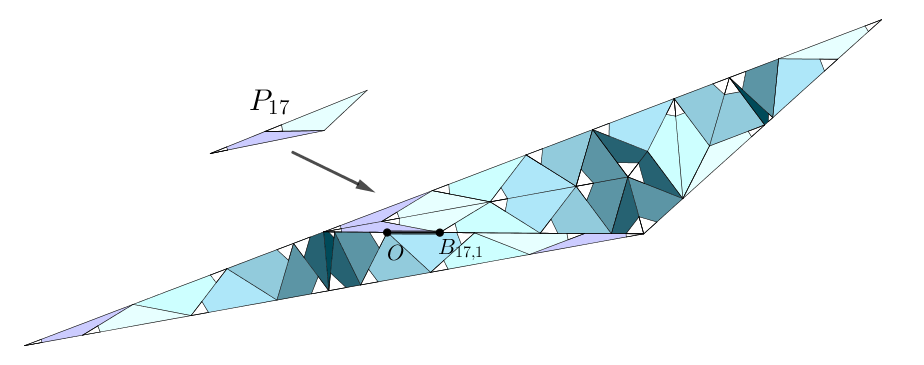
\includegraphics[width=0.8\textwidth]{ILCFig15_n=17}\\
\raggedright
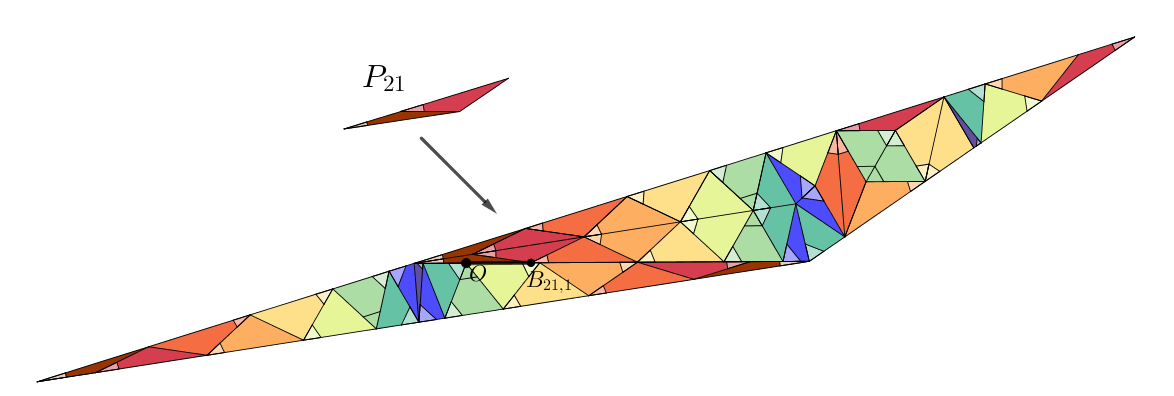
\includegraphics[width=1\textwidth]{ILCFig15_n=21}
			\caption{The segments $\overline{OB_{n,1}}, n\in \{17,21\}$.}
\label{fig:misfitn=1721}
\end{figure}

\begin{figure}[H]
\centering
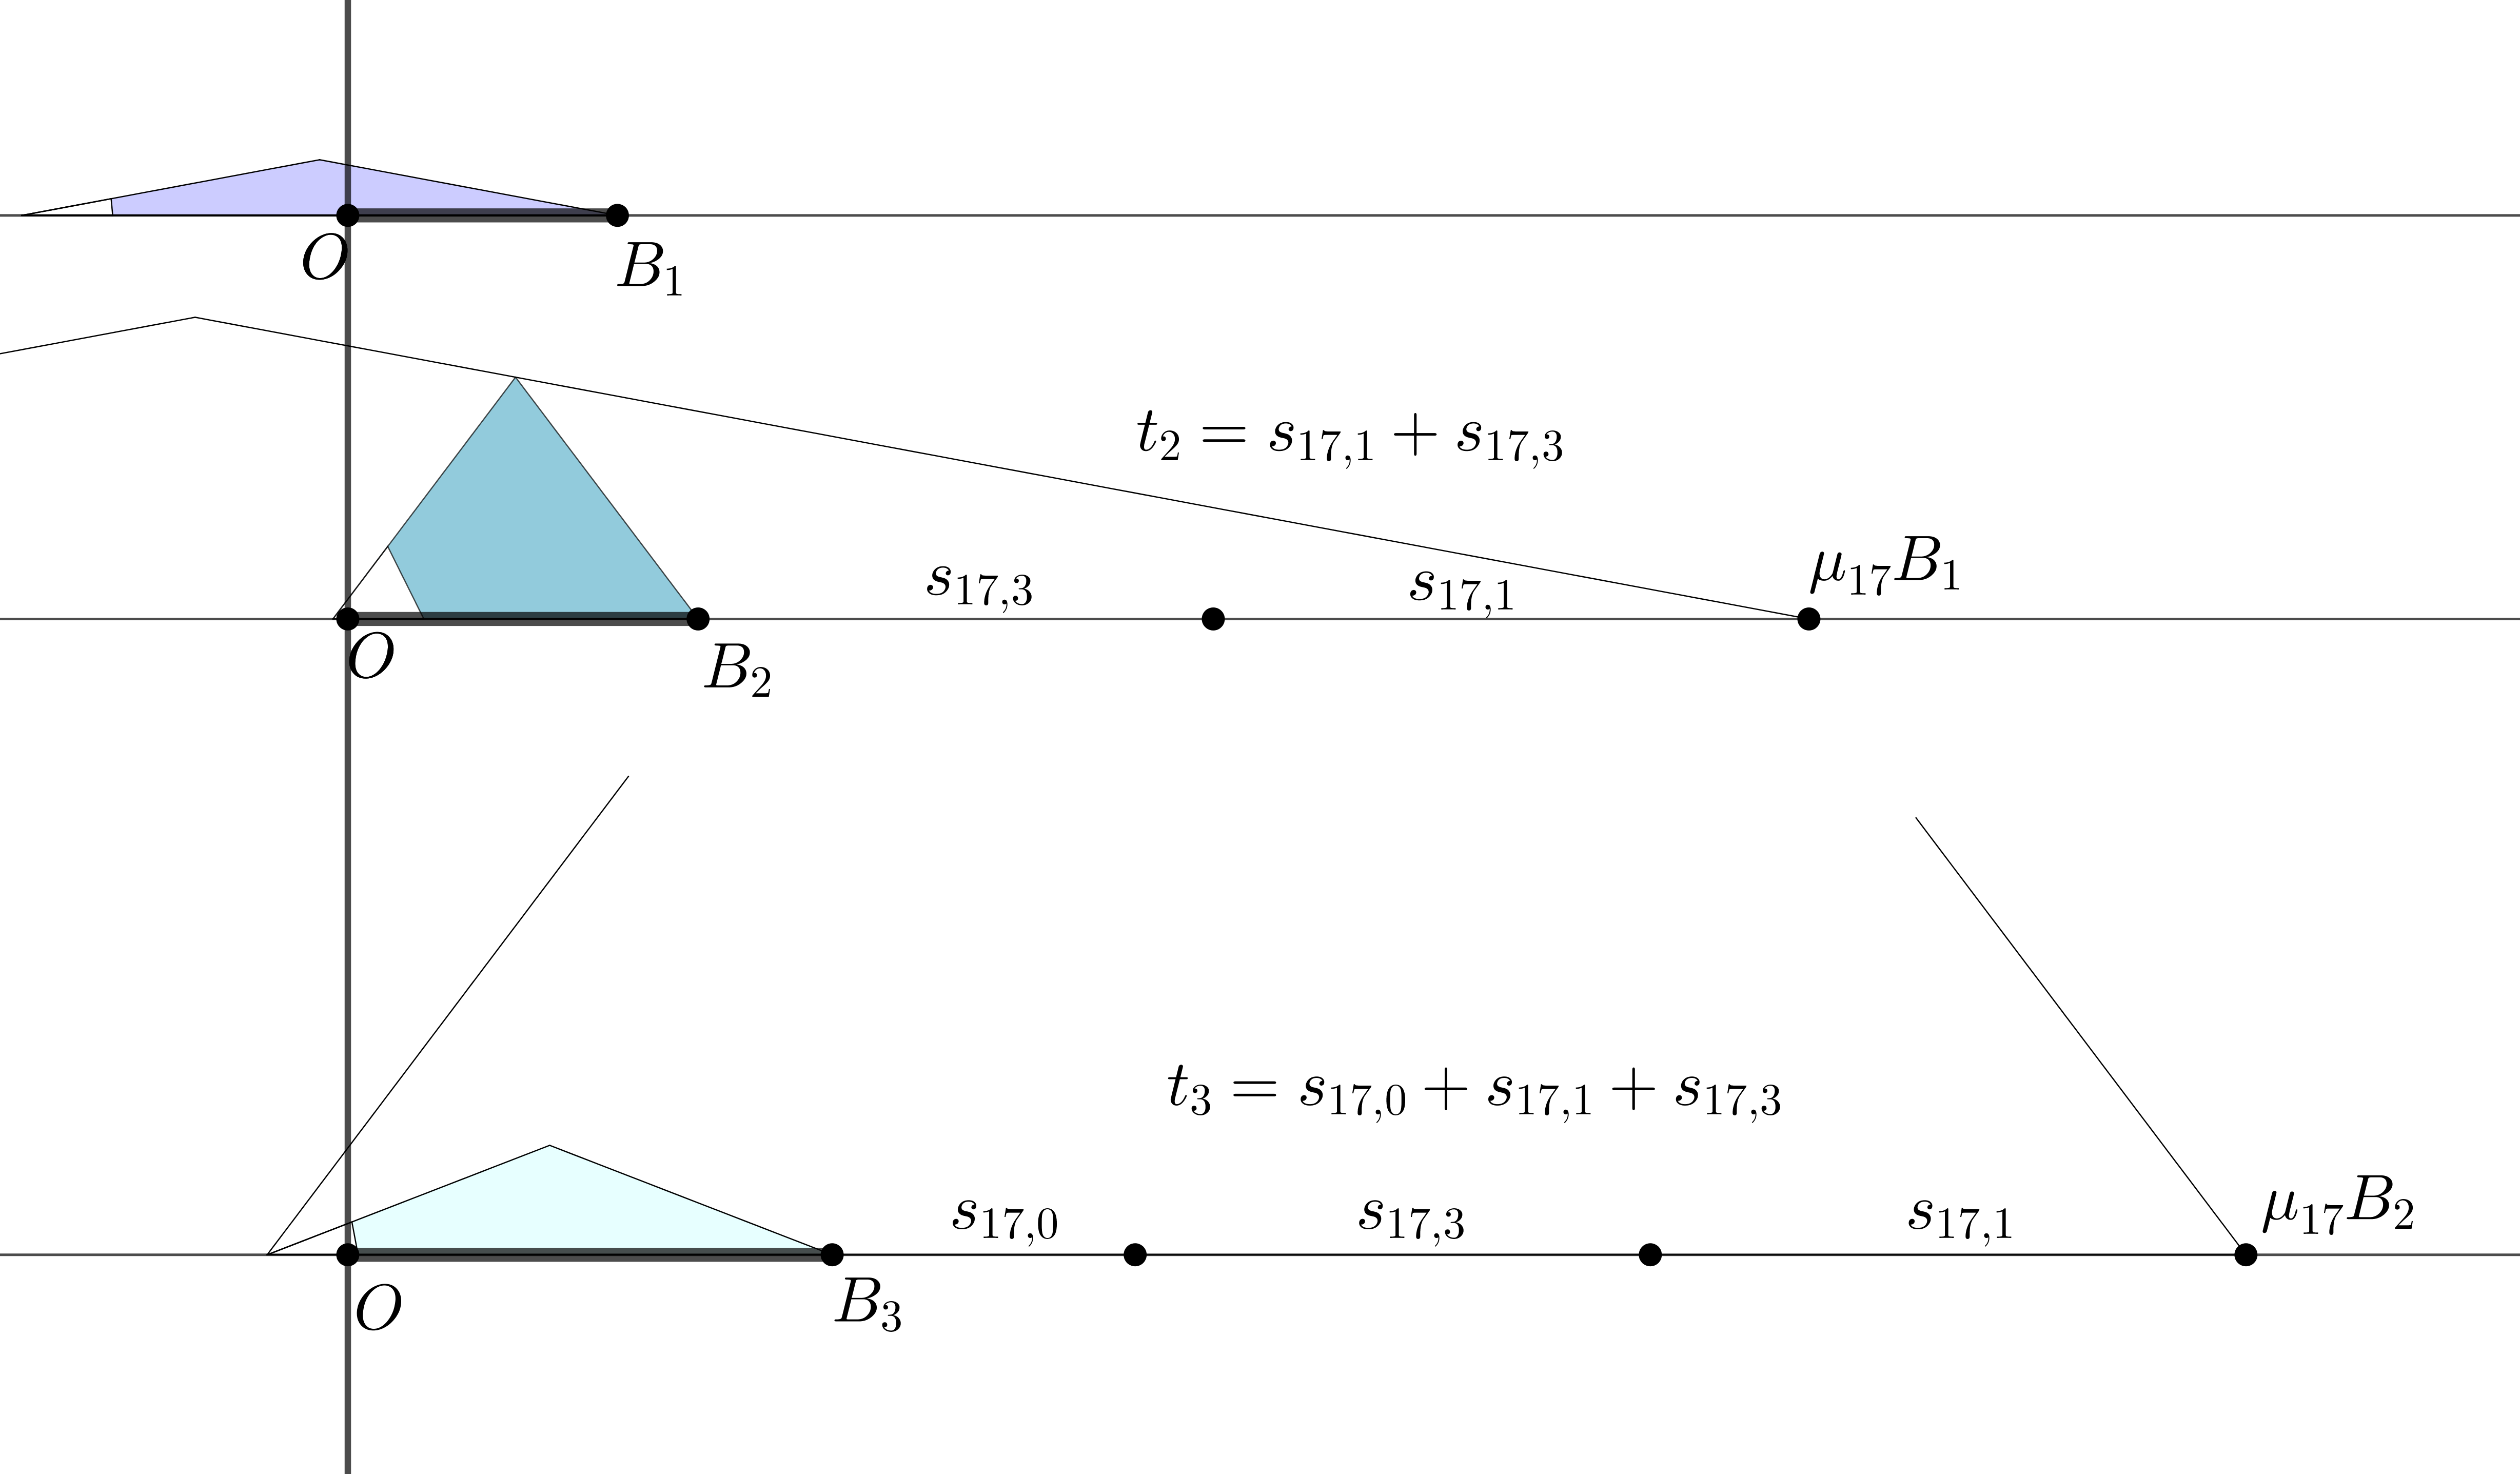
\includegraphics[width=0.8\textwidth]{ILCFig16_n=17_edges}
\caption{The segments $\overline{OB_{17,r,1}}, r=1,2,3$.}
\label{fig:n=17nonflc}
\end{figure}

\begin{figure}[H]
\centering
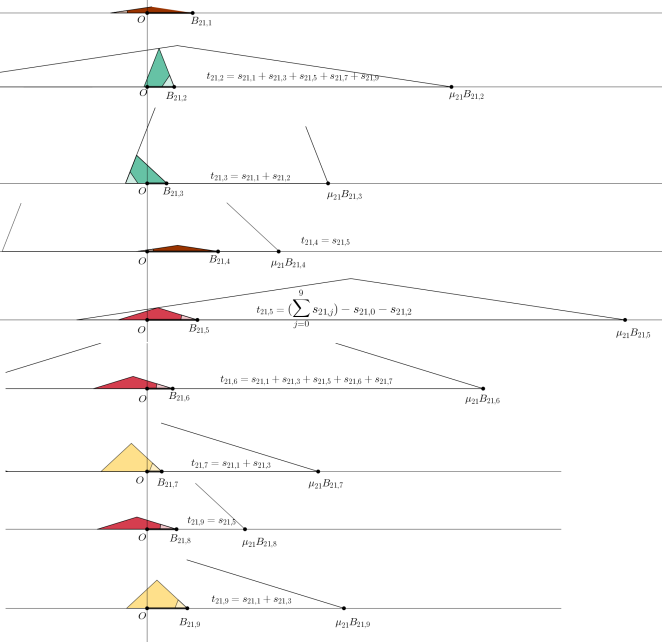
\includegraphics[width=1\textwidth]{ILCFig17_n=21_edges}
\caption{The segments $\overline{OB_{21,r,1}}, r=1,2,\ldots,9$.}
\label{fig:n=21nonflc}
\end{figure}
			
			